\section{Additional Figures and Tables}
\label{sec:appendix_more}

This appendix contains secondary charts and tables referenced by the main paper. They are included to preserve traceability while keeping the main paper focused on RQ1--RQ4.

\subsection{Controlled Term Recovery}

\begin{figure}[h]
\centering
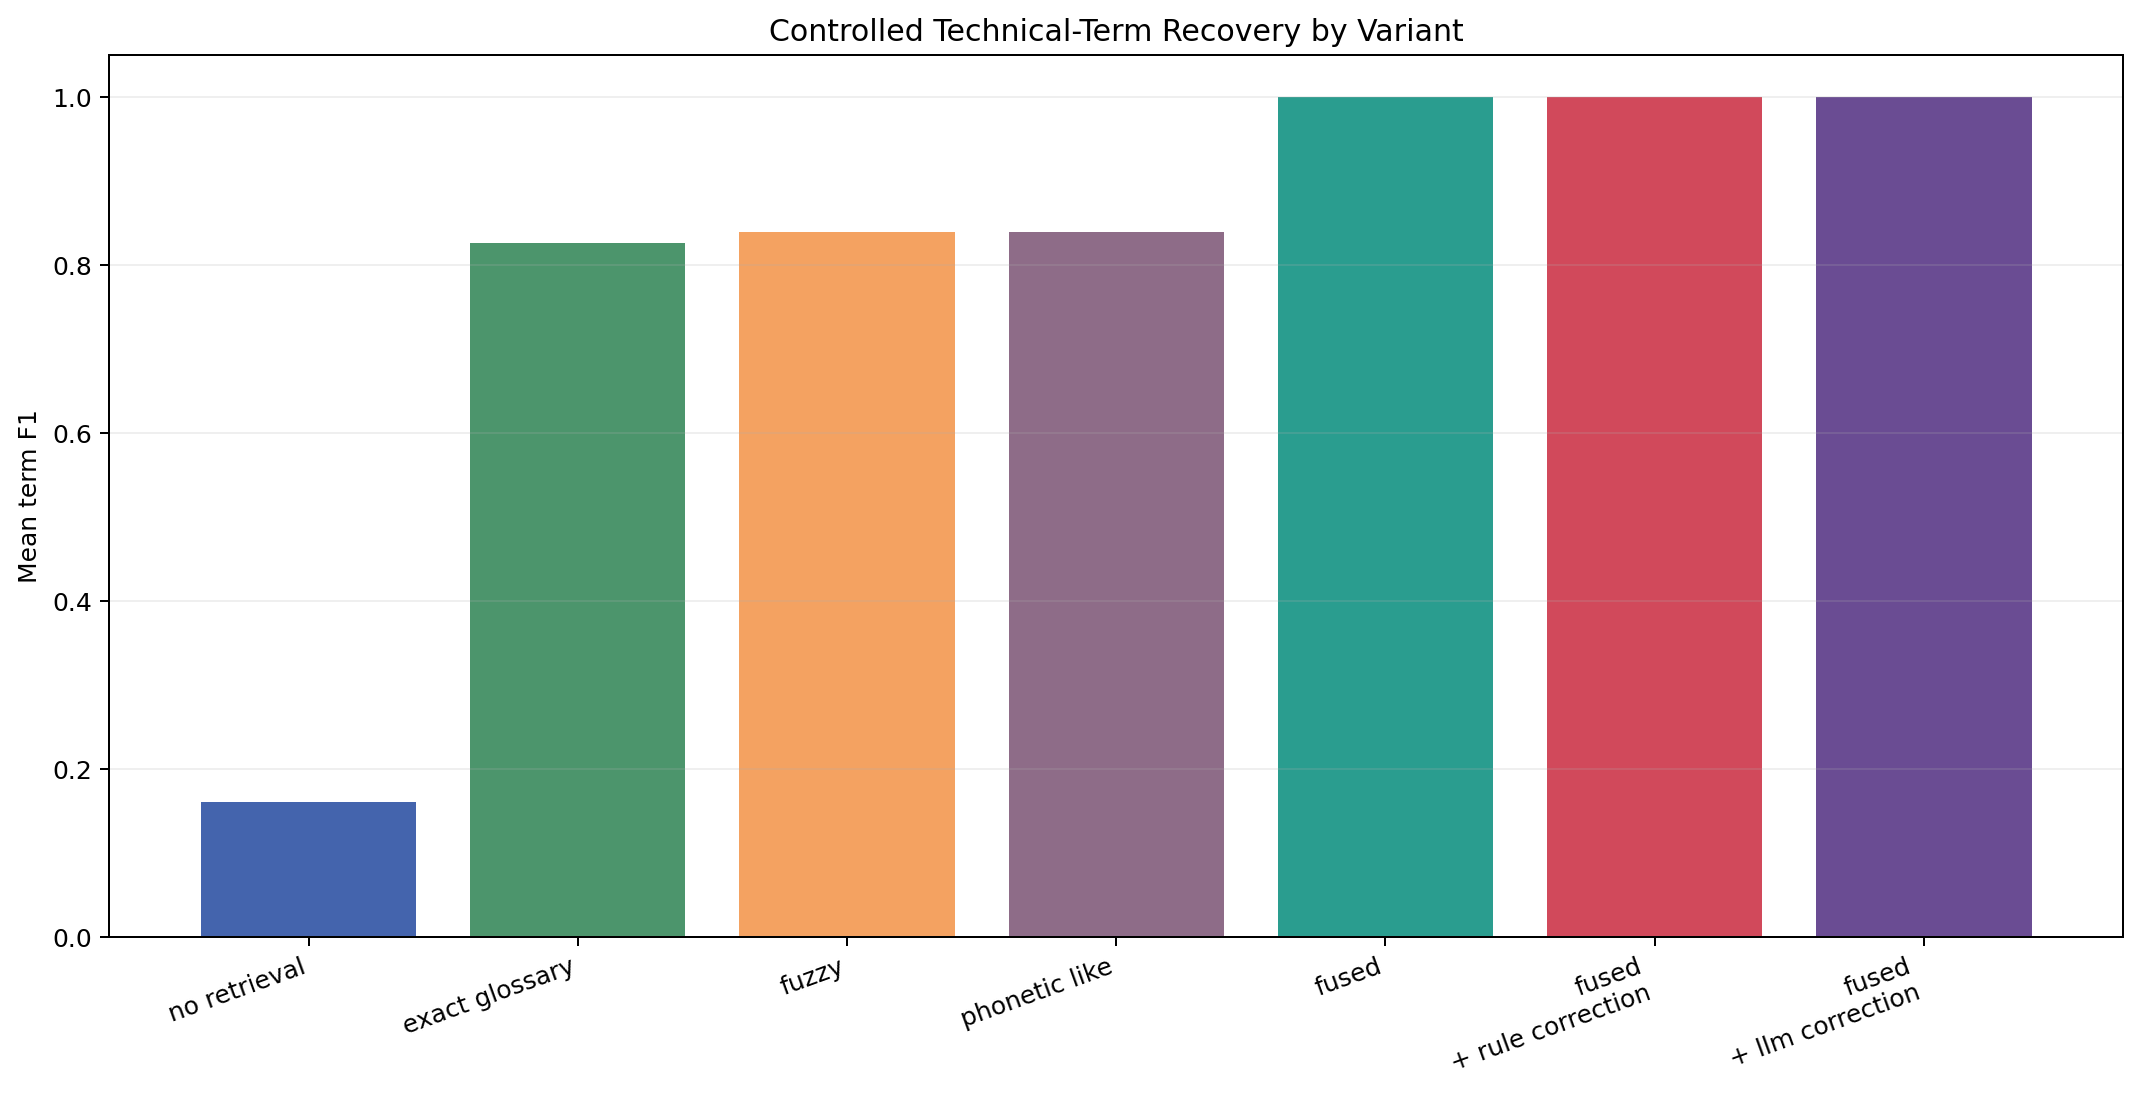
\includegraphics[width=\columnwidth]{figures/term_rescue_f1_by_variant.png}
\caption{Controlled term-rescue F1 by variant. These are text-fixture results; they support mechanism testing only. Exact source paths are listed in the manifest and claim audit.}
\label{fig:app_term_f1}
\end{figure}

\begin{table}[h]
\centering
\scriptsize
\begin{tabular}{llrrrr}
\toprule
Variant & Group & Cases & Term F1 & Error after & Review \\
\midrule
no retrieval & en easy & 7 & 0.000 & 0.218 & 0 \\
fused & en hard & 5 & 1.000 & 0.351 & 0 \\
fused+rule & en hard & 5 & 1.000 & 0.000 & 0 \\
fused+LLM & en hard & 5 & 1.000 & 0.223 & 2 \\
fused+rule & negative control & 4 & 1.000 & 0.000 & 4 \\
\bottomrule
\end{tabular}
\caption{Selected controlled term-rescue rows. The negative-control review count is a safety behavior, not a public-audio performance claim.}
\label{tab:app_term_rows}
\end{table}

\subsection{Controlled Overlap Safety}

\begin{figure}[h]
\centering
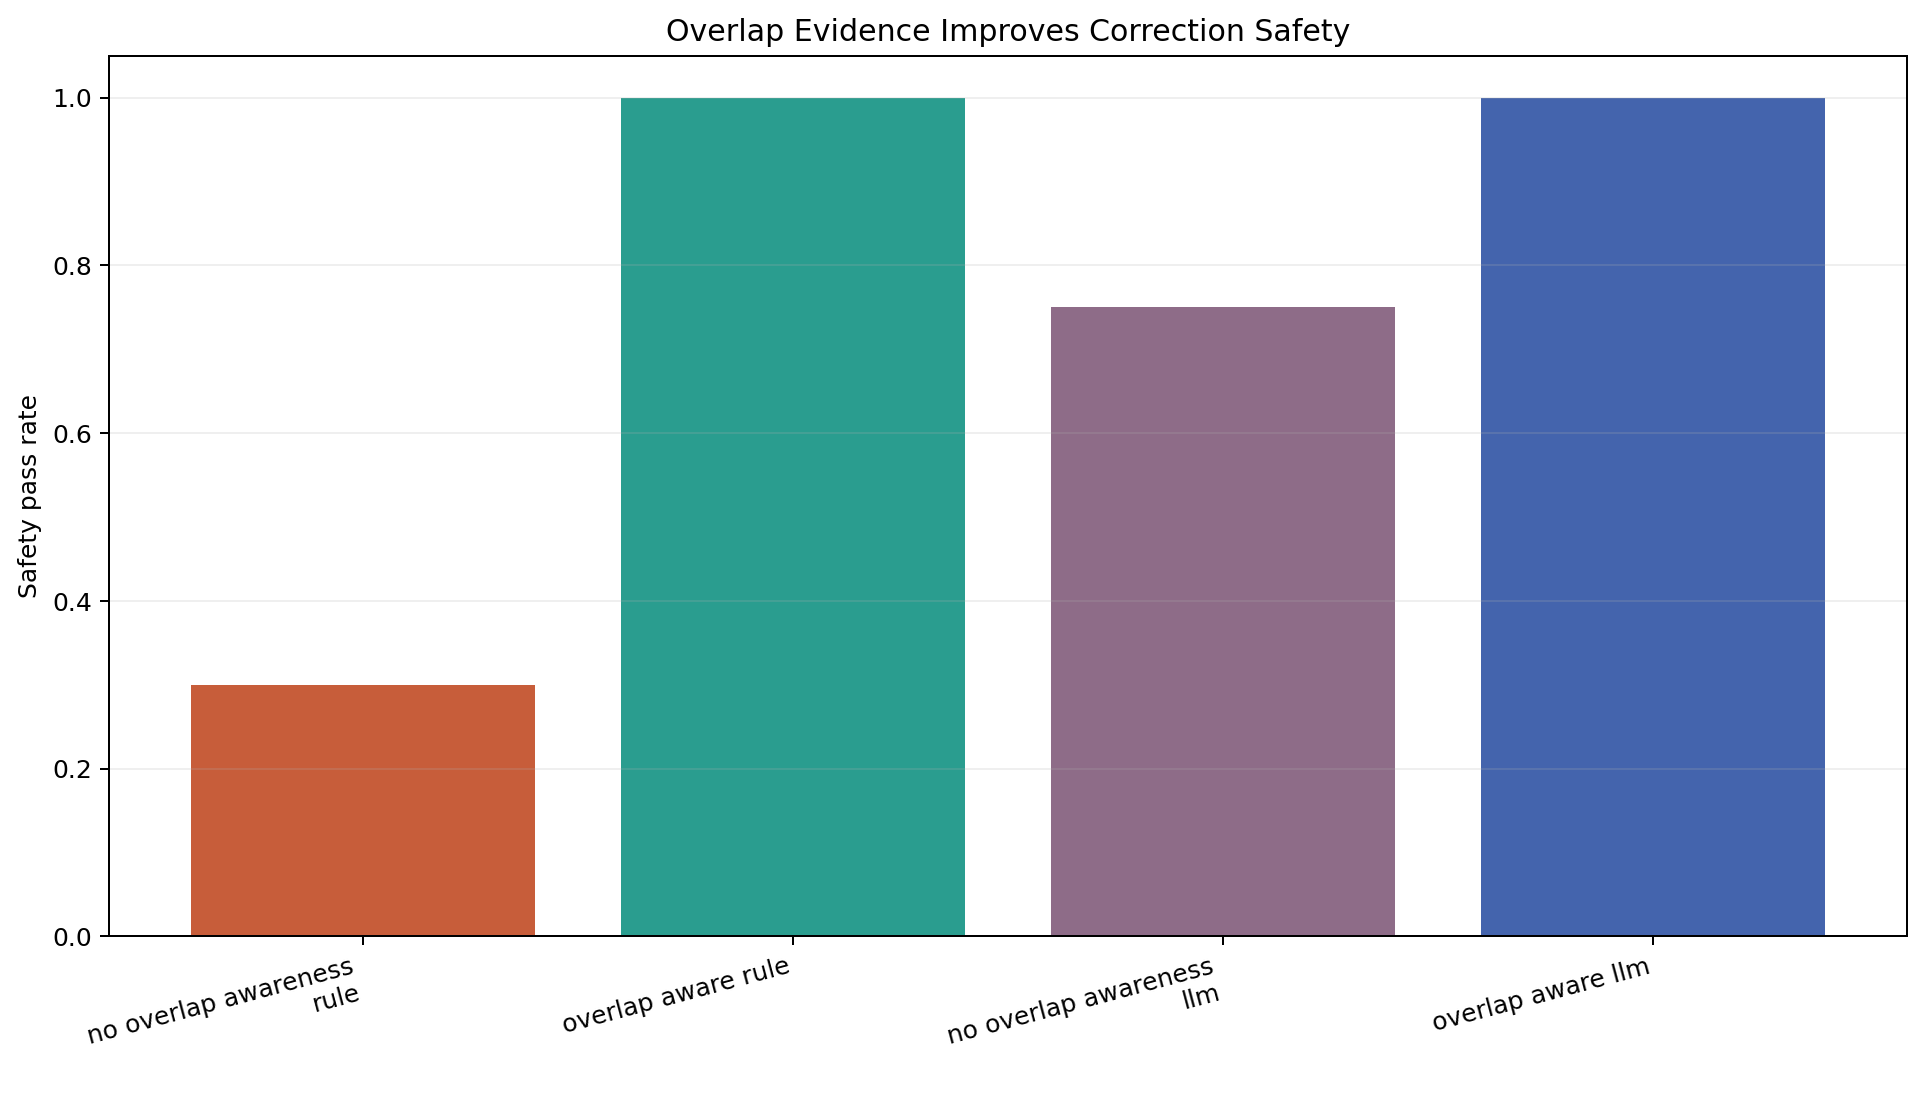
\includegraphics[width=\columnwidth]{figures/overlap_safety_pass_rate.png}
\caption{Controlled overlap safety pass rate generated from the controlled overlap summary.}
\label{fig:app_overlap_safety}
\end{figure}

\begin{table}[h]
\centering
\scriptsize
\begin{tabular}{llrrrr}
\toprule
Variant & True overlap & Uncertainty & Cases & Safety pass & Forbidden \\
\midrule
overlap-aware rule & true & high & 4 & 1.000 & 0 \\
overlap-aware LLM & true & high & 4 & 1.000 & 0 \\
no-overlap rule & true & high & 4 & 0.000 & 3 \\
no-overlap LLM & true & high & 4 & 0.500 & 0 \\
\bottomrule
\end{tabular}
\caption{Selected high-overlap controlled safety rows.}
\label{tab:app_overlap_rows}
\end{table}

\subsection{EvidenceGate Leakage and Held-out Failure}

\begin{figure}[h]
\centering
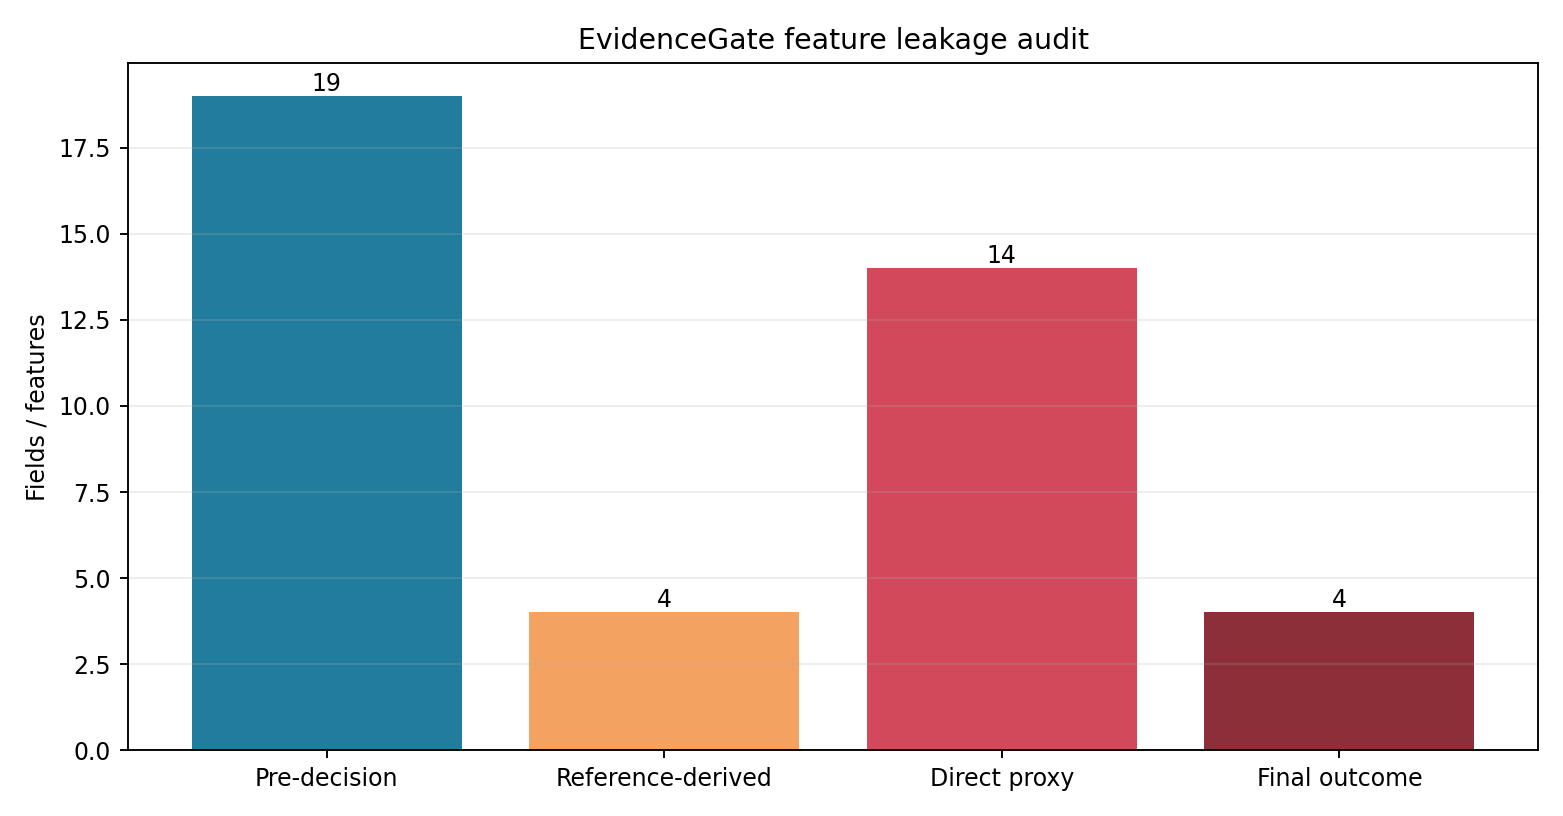
\includegraphics[width=\columnwidth]{figures/evidence_gate_feature_leakage_audit.png}
\caption{EvidenceGate feature leakage audit. The source document reports 41 audited fields: 19 allowed pre-decision, 4 risky reference-derived, 14 direct label proxy, and 4 final audit outcome fields.}
\label{fig:app_evidence_leakage}
\end{figure}

\begin{figure}[h]
\centering
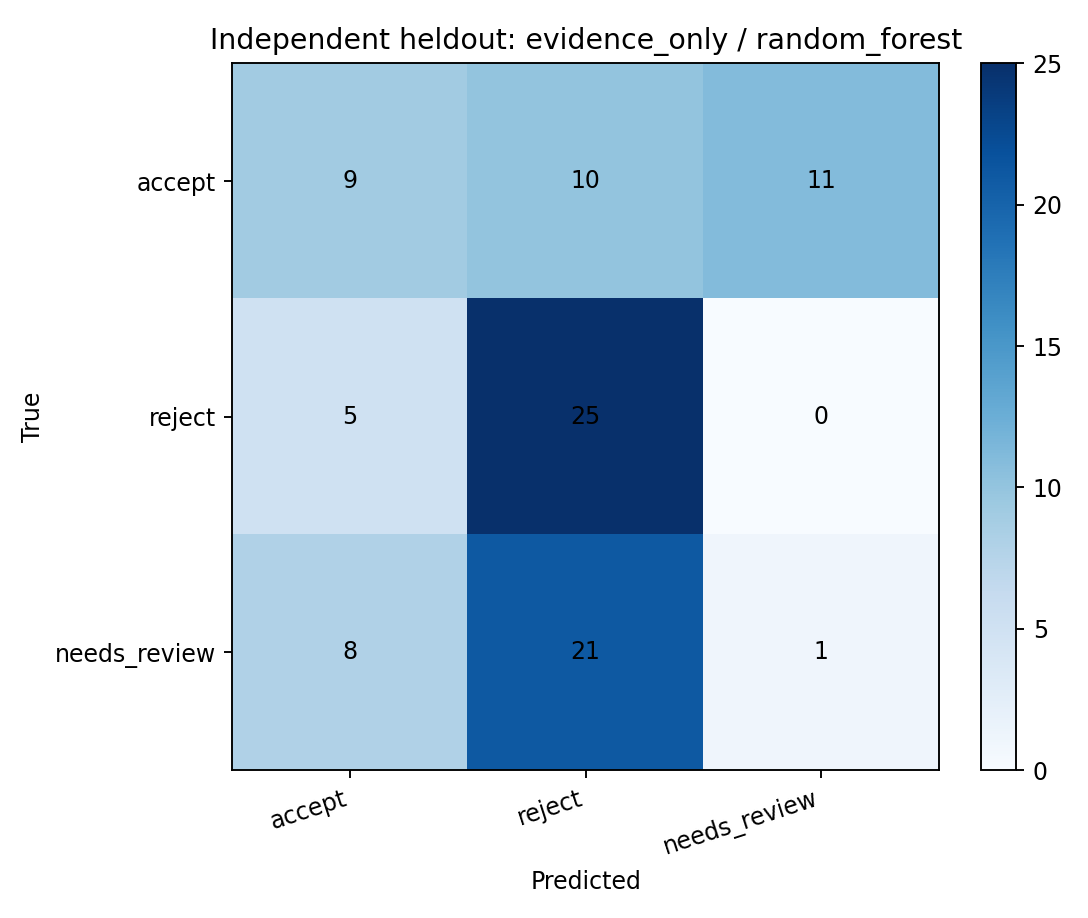
\includegraphics[width=\columnwidth]{figures/evidence_gate_heldout_confusion_matrix.png}
\caption{Independent held-out EvidenceGate confusion matrix. The associated metrics show weak generalization, especially for needs-review routing.}
\label{fig:app_evidence_confusion}
\end{figure}

\begin{table}[h]
\centering
\scriptsize
\begin{tabular}{llrrrr}
\toprule
Feature/model & Split & Macro F1 & False accept & Unsafe accept & Review recall \\
\midrule
audit-aware RF & grouped & 1.000 & 0.000 & 0.000 & 1.000 \\
evidence-only RF & grouped & 0.976 & 0.000 & 0.000 & 0.962 \\
risk-only RF & grouped & 0.924 & 0.133 & 0.000 & 0.769 \\
evidence-only RF & independent & 0.325 & 0.217 & 0.167 & 0.033 \\
evidence-only LR & independent & 0.316 & 0.100 & 0.067 & 0.000 \\
\bottomrule
\end{tabular}
\caption{EvidenceGate validation rows from the EvidenceGate metrics CSV and document. The audit-aware grouped result is a policy-distillation sanity check.}
\label{tab:app_evidence_gate}
\end{table}

\subsection{Binary Safe-to-Apply Stress Test}

\begin{figure}[h]
\centering
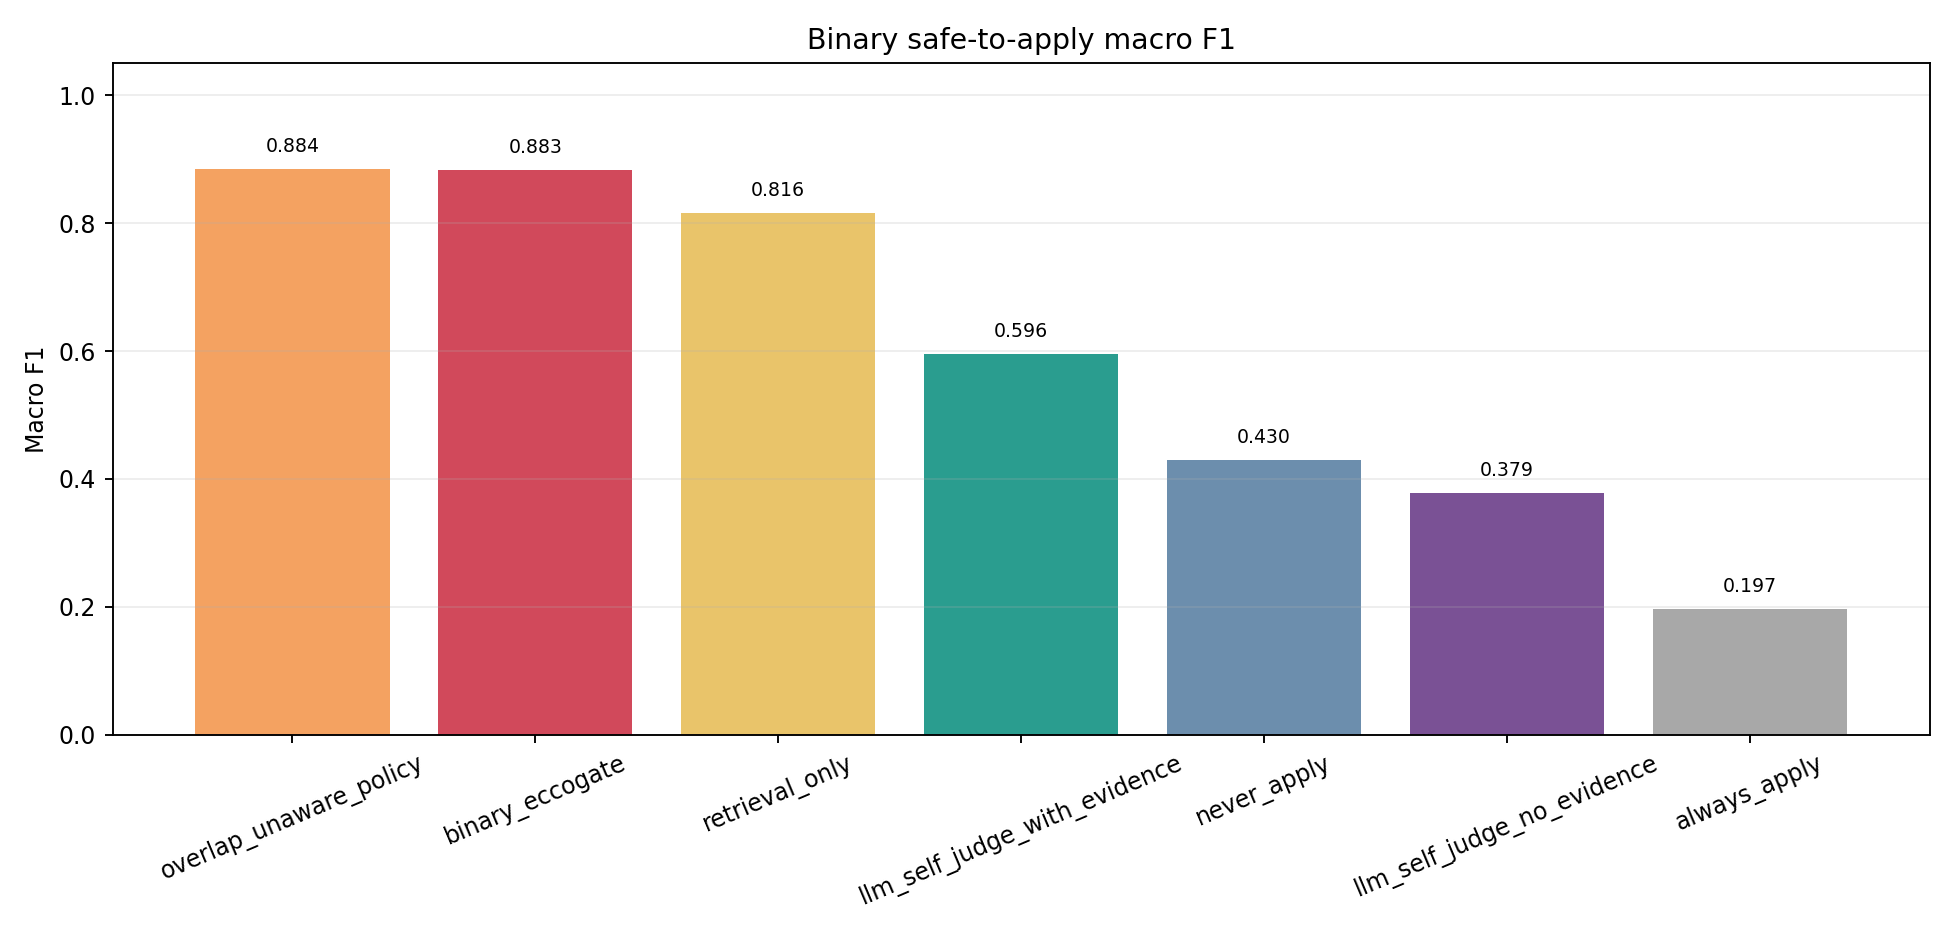
\includegraphics[width=\columnwidth]{figures/binary_safe_apply_macro_f1.png}
\caption{Binary safe-to-apply macro F1. The benchmark is controlled/pilot, not real-audio generalization.}
\label{fig:app_binary_f1}
\end{figure}

\begin{table}[h]
\centering
\scriptsize
\begin{tabular}{lrrrr}
\toprule
Method & Examples & Macro F1 & Unsafe apply & Coverage \\
\midrule
always apply & 327 & 0.197 & 1.000 & 1.000 \\
retrieval only & 327 & 0.816 & 0.198 & 0.385 \\
overlap-unaware policy & 327 & 0.884 & 0.077 & 0.272 \\
binary EccoGate & 327 & 0.883 & 0.053 & 0.239 \\
LLM judge with evidence & 327 & 0.596 & 0.324 & 0.385 \\
\bottomrule
\end{tabular}
\caption{Selected binary safe-to-apply rows.}
\label{tab:app_binary}
\end{table}

\subsection{Interruption Candidate Review}

\begin{table}[h]
\centering
\scriptsize
\begin{tabular}{lrrrrr}
\toprule
Candidates & Reviewed & Interruption & Other labels & Precision & Recall/F1 \\
\midrule
10 & 10 & 10 & 0 & 1.000 & unavailable \\
\bottomrule
\end{tabular}
\caption{Human-reviewed interruption candidate summary. Precision is candidate precision only; recall and F1 are unavailable.}
\label{tab:app_interruption}
\end{table}

\subsection{Runtime and Mobile-Style Evidence}

\begin{figure}[h]
\centering

\includegraphics[width=\columnwidth]{figures/asr_rtf_by_model.png}
\caption{ASR real-time factor chart. This figure supports local runtime trade-off discussion only.}
\label{fig:app_rtf}
\end{figure}

\begin{table}[h]
\centering
\scriptsize
\begin{tabular}{llrrrr}
\toprule
Dataset & Model & Rows & Error & Cleaned error & RTF \\
\midrule
AMI & tiny & 8 & 0.382 & 0.314 & 0.031 \\
AMI & base & 8 & 0.351 & 0.280 & 0.056 \\
FLEURS en & tiny & 10 & 0.186 & 0.186 & 0.072 \\
FLEURS en & base & 10 & 0.134 & 0.134 & 0.140 \\
\bottomrule
\end{tabular}
\caption{Selected local-machine whisper.cpp Level 1 rows. These are not phone-device measurements.}
\label{tab:app_mobile}
\end{table}
